\documentclass[]{article}
\usepackage{listings} 
\usepackage{algorithm}
\usepackage{algorithmic}
\usepackage{graphicx}
\graphicspath{ {images/} }
\usepackage{float}
\usepackage{geometry}
\usepackage{pdfpages}

%opening
\title{}
\author{}
\date{}
\special{papersize=8.5in,11in}
\geometry{left=1.5cm,right=2cm,top=1.5cm,bottom=1.5cm}

\begin{document}
	
	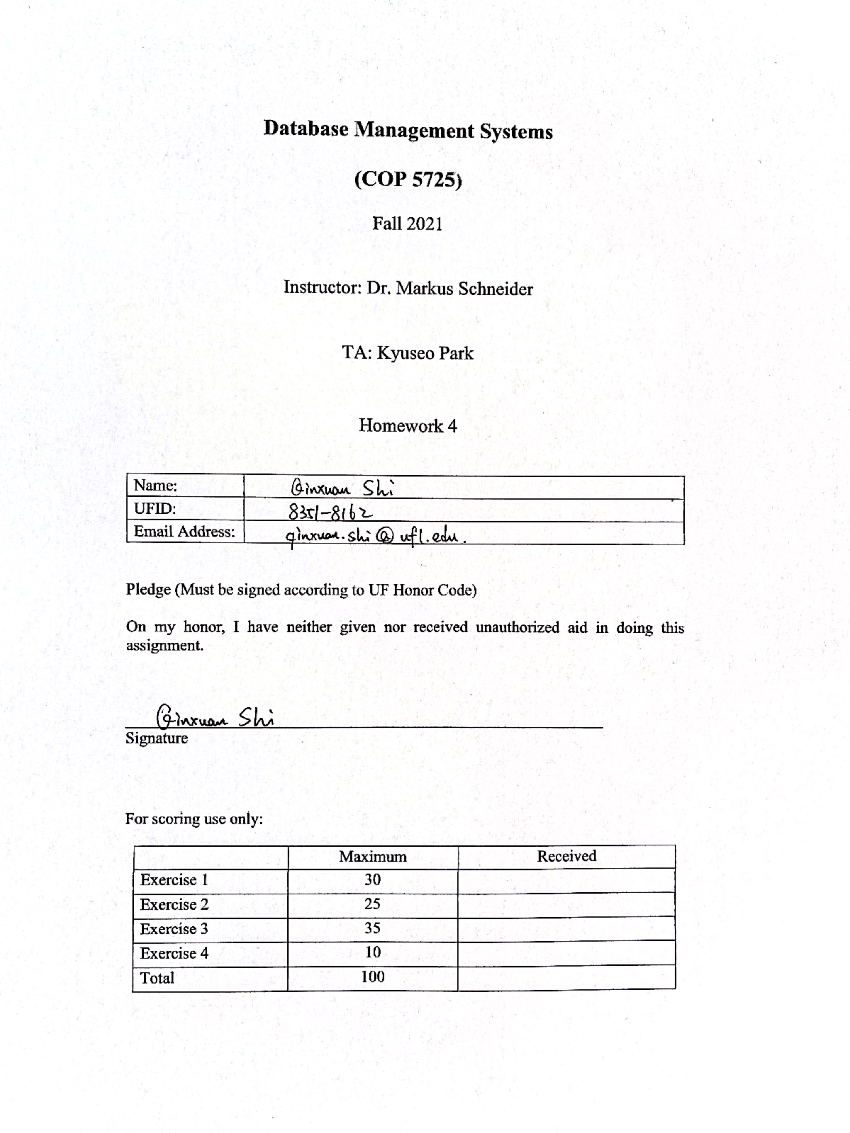
\includepdf{../HW4.pdf}
	
	\section{Exercise 1}
	
	1. [5 points] Use the Armstrong axioms to prove the soundness of the Union rule. If A → B and A → C holds, then A → BC holds. \\
	
	\noindent Now we have already know that $A\rightarrow B$ and $A\rightarrow C$. Firstly, using Augmentation rule to first FD, we can get $AA\rightarrow AB$, which is $A\rightarrow AB$ since $AA = A$. Secondly, also use Augmentation rule to second FD, we can get $AB\rightarrow BC$. Finally, we use Transitivity rule, and we can know that $A\rightarrow BC$. Because the Augmentation rule and Transitivity rule have been shown that they are sound and complete, so the Union rule can also fulfill the Soundness.  \\
	
	\noindent 2. [4 points, 2 points each] Given the set F = {A→B, AB→C, AC→BD} of functional dependencies, prove the following dependencies by using the Armstrong axioms.   \\
	
	(1) A→ABC  \\
	
	Augmentation rule: $A\rightarrow B \Longrightarrow A\rightarrow AB$ and $AB\rightarrow C \Longrightarrow AB\rightarrow BC$  \\
	
	Transitivity rule: $AB\rightarrow BC$, $A\rightarrow AB$ $\Longrightarrow$  $A\rightarrow BC$   \\
	
	Then, we use Augmentation rule for $A\rightarrow BC$, we finally get $AA\rightarrow ABC$, which is actually $A\rightarrow ABC$ \\
	
	(2) AD→BCD  \\
	
	Augmentation rule: $A\rightarrow B \Longrightarrow AD\rightarrow BD$ and $A\rightarrow B \Longrightarrow A\rightarrow AB$  \\
	
	Transitivity rule: $AB\rightarrow C$, $A\rightarrow AB$ $\Longrightarrow$  $A\rightarrow C$   \\
	
	Augmentation rule: $A\rightarrow C$ $\Longrightarrow$  $AD\rightarrow CD$   \\
	
	Augmentation rule: $AD\rightarrow BD \Longrightarrow AD\rightarrow ABD$ and $AD\rightarrow CD \Longrightarrow ABD\rightarrow BCD$  \\
	
	Transitivity rule: $AD\rightarrow ABD$, $ABD\rightarrow BCD$ $\Longrightarrow$  $AD\rightarrow BCD$   \\
	
	\noindent 3. [6 points] Consider a relation schema R(X, Y, Z) with the functional dependencies XY→Z and Z→X. Can we conclude that Y→XZ holds? If yes, please argue why. If no, please argue why not by giving a counterexample.  \\
	
	\noindent We cannot conclude that  Y→XZ holds. It's easy to know that $Y^{+} = Y$, and $XZ \not\subseteq Y$, so we cannot get the statement.   \\
	
	\noindent For example, suppose that X represents students name and all of these names are distinct, Y represents gender, Z represents student ID as UFID. Since names of students are all different, it is easy to know that $X\rightarrow Z$ holds and $XY\rightarrow Z$ holds too. we can also know that $Z\rightarrow X$ holds. However, to the statement $Y\rightarrow XZ$, it is impossible for the single gender attribute to determine name and ID functionally. As a result, we cannot conclude $Y\rightarrow XZ$ holds with the functional dependencies that given by the problem.   \\
	
	\noindent 4. [5 points] Consider the relation schema R(A, B, C, D, E, F) and the set of functional dependencies F = {A→B, A→C, CD→E, CD→F, B→E}. Infer at least five new FDs by using five different Armstrong’s axioms and derived inference rules. (Please do not include the trivial ones such as A→A in your answer.) Show each step.  \\
	
	(1) Transitivity rule: $A\rightarrow B$, $B\rightarrow E$ $\Longrightarrow$  $A\rightarrow E$   \\
	
	(2) Augmentation rule: $A\rightarrow C$ $\Longrightarrow$  $AB\rightarrow BC$   \\
	
	(3) Union rule: $A\rightarrow B$, $A\rightarrow C$ $\Longrightarrow$  $A\rightarrow BC$   \\
	
	(4) Decomposition rule: we can know that $AB\rightarrow BC$ from (2), then we can get $AB\rightarrow B$ and $AB\rightarrow C$   \\
	
	(5) Pseudotransitivity rule: $A\rightarrow C$, $CD\rightarrow E$ $\Longrightarrow$  $AD\rightarrow E$   \\
	
	(6) Pseudotransitivity rule: $A\rightarrow C$, $CD\rightarrow F$ $\Longrightarrow$  $AD\rightarrow F$   \\
	
	(7) Reflexivity rule: since $D\subseteq CD$, we can get $CD\rightarrow D$  \\
	
	\noindent 5. [10 points] Assume we have a set F = {A→B, C→D} of functional dependencies for a relation schema R(A, B, C, D). Write down all the functional dependencies of the closure F+ of F and count them.   \\
	
	\noindent Firstly, we can get the set of all sets that are subsets of R(A,B,C,D):  \\
	
	\{$\emptyset$,A,B,C,D,AB,AC,AD,BC,BD,CD,ABC,ABD,ACD,BCD,ABCD\} \\
	
	\noindent Then, we compute the attribute closures of all subsets except $\emptyset$.   \\
	
	$A^{+}$: AB  \\
	
	$\Longrightarrow$ $A\rightarrow A, A\rightarrow B, A\rightarrow AB$ (3FDs)  \\
	
	$B^{+}$: B  \\
	
	$\Longrightarrow$ $B\rightarrow B$ (1FDs)  \\
	
	$C^{+}$: CD  \\
	
	$\Longrightarrow$ $C\rightarrow C, C\rightarrow D, C\rightarrow CD$ (3FDs)  \\
	
	$D^{+}$: D  \\
	
	$\Longrightarrow$ $D\rightarrow D$ (1FDs)  \\
	
	$AB^{+}$: AB  \\
	
	$\Longrightarrow$ $AB\rightarrow A, AB\rightarrow B, AB\rightarrow AB$ (3FDs)  \\
	
	$AC^{+}$: ABCD  \\
	
	$\Longrightarrow$ $AC\rightarrow A, AC\rightarrow B, AC\rightarrow C, AC\rightarrow D, AC\rightarrow AB, AC\rightarrow AC, AC\rightarrow AD, AC\rightarrow BC, AC\rightarrow BD, AC\rightarrow CD, AC\rightarrow ABC, AC\rightarrow ABD, AC\rightarrow ACD, AC\rightarrow BCD, AC\rightarrow ABCD$ (15FDs)  \\
	
	$AD^{+}$: ABD  \\
	
	$\Longrightarrow$ $AD\rightarrow A, AD\rightarrow B, AD\rightarrow D, AD\rightarrow AB, AD\rightarrow AD, AD\rightarrow BD, AD\rightarrow ABD$ (7FDs)  \\
	
	$BC^{+}$: BCD  \\
	
	$\Longrightarrow$ $BC\rightarrow B, BC\rightarrow C, BC\rightarrow D, BC\rightarrow BC, BC\rightarrow BD, BC\rightarrow CD, BC\rightarrow BCD$ (7FDs)  \\
	
	$BD^{+}$: BD  \\
	
	$\Longrightarrow$ $BD\rightarrow B, BD\rightarrow D, BD\rightarrow BD$ (3FDs)  \\
	
	$CD^{+}$: CD  \\
	
	$\Longrightarrow$ $CD\rightarrow C, CD\rightarrow D, CD\rightarrow CD$ (3FDs)  \\
	
	$ABC^{+}$: ABCD  \\
	
	$\Longrightarrow$ $ABC\rightarrow A, ABC\rightarrow B, ABC\rightarrow C, ABC\rightarrow D, ABC\rightarrow AB, ABC\rightarrow AC, ABC\rightarrow AD, ABC\rightarrow BC, ABC\rightarrow BD, ABC\rightarrow CD, ABC\rightarrow ABC, ABC\rightarrow ABD, ABC\rightarrow ACD, ABC\rightarrow BCD, ABC\rightarrow ABCD$ (15FDs)  \\
	
	$ABD^{+}$: ABD  \\
	
	$\Longrightarrow$ $ABD\rightarrow A, ABD\rightarrow B, ABD\rightarrow D, ABD\rightarrow AB, ABD\rightarrow AD, ABD\rightarrow BD, ABD\rightarrow ABD$ (7FDs)  \\
	
	$ACD^{+}$: ABCD  \\
	
	$\Longrightarrow$ $ACD\rightarrow A, ACD\rightarrow B, ACD\rightarrow C, ACD\rightarrow D, ACD\rightarrow AB, ACD\rightarrow AC, ACD\rightarrow AD, ACD\rightarrow BC, ACD\rightarrow BD, ACD\rightarrow CD, ACD\rightarrow ABC, ACD\rightarrow ABD, ACD\rightarrow ACD, ACD\rightarrow BCD, ACD\rightarrow ABCD$ (15FDs)  \\
	
	$BCD^{+}$: BCD  \\
	
	$\Longrightarrow$ $BCD\rightarrow B, BCD\rightarrow C, BCD\rightarrow D, BCD\rightarrow BC, BCD\rightarrow BD, BCD\rightarrow CD, BCD\rightarrow BCD$ (7FDs)  \\
	
	$ABCD^{+}$: ABCD  \\
	
	$\Longrightarrow$ $ABCD\rightarrow A, ABCD\rightarrow B, ABCD\rightarrow C, ABCD\rightarrow D, ABCD\rightarrow AB, ABCD\rightarrow AC, ABCD\rightarrow AD, ABCD\rightarrow BC, ABCD\rightarrow BD, ABCD\rightarrow CD, ABCD\rightarrow ABC, ABCD\rightarrow ABD, ABCD\rightarrow ACD, ABCD\rightarrow BCD, ABCD\rightarrow ABCD$ (15FDs)  \\
	
	\noindent To conclude, the closure $F^{+}$ of F has 105 elements. \\
	
	\section{Exercise 2}
	
	1. [5 points] Consider the relation schema R = (A, B, C, D, E, F, G, H) with the set of functional dependencies K = {A→B, B→G, AC→D, DF→E, FG→BH}. Show for each of the following FDs whether they can be inferred from K.   \\
	
	(1) ABD→ACE  \\
	
	Compute $ABD^{+}$, and we can get $ABD^{+}$:ABDG. $ACE\not\subseteq ABDG$, so $ABD\rightarrow ACE$ cannot be inferred from K.   \\
	
	(2) BFG→BEFG   \\
	
	Compute $BFG^{+}$, and we can get $BFG^{+}$:BFGH. $BEFG\not\subseteq BFGH$, so $BFG\rightarrow BEFG$ cannot be inferred from K.   \\
	
	(3) ABF→ABDG   \\
	
	Compute $ABF^{+}$, and we can get $ABF^{+}$:ABFGH. $ABDG\not\subseteq ABFGH$, so $ABF\rightarrow ABDG$ cannot be inferred from K.   \\
	
	(4) CEG→BCEF   \\
	
	Compute $CEG^{+}$, and we can get $CEG^{+}$:CEG. $BCEF\not\subseteq CEG$, so $CEG\rightarrow BCEF$ cannot be inferred from K.   \\
	
	\noindent 2. [5 points] Consider the relation schema R(A, B, C, D, E, F, G, H) with functional dependencies F = {A→C, AC→E, D→EH, F→G} and G = {A→BCE, AD→CFG, D→A, DE→GH, F→D}. Are the two sets F and G equivalent? Show each step.  \\
	
	\noindent Firstly, we show every FD in F can be inferred from G.  \\
	
	\noindent F has the left-hand sides A, AC, D and F.  \\
	
	\noindent With respect to G we calculate $A^{+}, AC^{+}, D^{+} and F^{+}$, and we get $A^{+} = ABCE$, $AC^{+} = ABCE$, $D^{+} = ABCDEFGH$, $F^{+} = ABCDEFGH$.    \\
	
	\noindent We check whether the right-hand sides of the FDs in F are in the respective attribute closures just computed for their left-hand sides:  \\
	
	\noindent $A\rightarrow C: C\subseteq A^{+}$ holds, $AC\rightarrow E: E\subseteq AC^{+}$ holds, $D\rightarrow EH: EH\subseteq D^{+}$ holds, $F\rightarrow G: G\subseteq F^{+}$ holds.   \\
	
	\noindent Secondly, we show every FD in G can be inferred from F.  \\
	
	\noindent G has the left-hand sides A, AD, D, DE and F.  \\
	
	\noindent With respect to F we calculate $A^{+}, AD^{+}, D^{+}, DE^{+} and F^{+}$, and we get $A^{+} = ACE$, $AD^{+} = ACDEH$, $D^{+} = DEH$, $DE^{+} = DEH$, $F^{+} = FG$.    \\
	
	\noindent We check whether the right-hand sides of the FDs in G are in the respective attribute closures just computed for their left-hand sides:  \\
	
	\noindent $A\rightarrow BCE: BCE\not\subseteq A^{+}$, $AD\rightarrow CFG: CFG\not\subseteq AD^{+}$, $D\rightarrow A: A\not\subseteq D^{+}$, $DE\rightarrow GH: GH\not\subseteq DE^{+}$, $F\rightarrow D: D\not\subseteq F^{+}$.   \\
	
	\noindent We can know that G covers F while F cannot cover G, as a result, two sets F and G are not equivalent.  \\
	
	\noindent 3. [5 points] Consider the relation schema R(A, B, C, D, E, F) with the functional dependencies K = {A→B, BD→E, AC→F, DE→C}. Which of the following attribute sets is a key? Show each step.  \\
	
	(1) ABCE  \\
	
	$ABCE^{+}$:= ABCE,   \\
	
	$A\rightarrow B$, $A\subseteq ABCE^{+}$ $\Longrightarrow$ $ABCE^{+}$:= ABCE \\
	
	$BD\rightarrow E$, $BD\not\subseteq ABCE^{+}$ $\Longrightarrow$ $ABCE^{+}$:= ABCE \\
	
	$AC\rightarrow F$, $AC\subseteq ABCE^{+}$  $\Longrightarrow$ $ABCE^{+}$:= ABCEF \\
	
	$DE\rightarrow C$, $DE\not\subseteq ABCE^{+}$  $\Longrightarrow$ $ABCE^{+}$:= ABCEF \\
	
	Because $ABCE^{+}\ne R$, ABCE is not a key.  \\
	
	(2) ABDF   \\
	
	$ABDF^{+}$:= ABDF,   \\
	
	$A\rightarrow B$, $A\subseteq ABDF^{+}$ $\Longrightarrow$ $ABDF^{+}$:= ABDF \\
	
	$BD\rightarrow E$, $BD\subseteq ABDF^{+}$ $\Longrightarrow$ $ABDF^{+}$:= ABDEF \\
	
	$AC\rightarrow F$, $AC\not\subseteq ABDF^{+}$  $\Longrightarrow$ $ABDF^{+}$:= ABDEF \\
	
	$DE\rightarrow C$, $DE\subseteq ABDF^{+}$  $\Longrightarrow$ $ABDF^{+}$:= ABCDEF \\
	
	$AC\rightarrow F$, $AC\subseteq ABDF^{+}$  $\Longrightarrow$ $ABDF^{+}$:= ABCDEF \\
	
	Because $ABDF^{+} = R$, ABDF is a super key.  \\
	
	Then we will figure out if there exist any L$\subset$ABDF$\rightarrow$R  \\
	
	We find that $AD^{+}$:= ABCDEF, so ABDF is just a super key, not a key.  \\
	
	(3) BEF    \\
	
	$BEF^{+}$:= BEF,   \\
	
	$A\rightarrow B$, $A\not\subseteq BEF^{+}$ $\Longrightarrow$ $BEF^{+}$:= BEF \\
	
	$BD\rightarrow E$, $BD\not\subseteq BEF^{+}$ $\Longrightarrow$ $BEF^{+}$:= BEF \\
	
	$AC\rightarrow F$, $AC\not\subseteq BEF^{+}$  $\Longrightarrow$ $BEF^{+}$:= BEF \\
	
	$DE\rightarrow C$, $DE\not\subseteq BEF^{+}$  $\Longrightarrow$ $BEF^{+}$:= BEF \\
	
	Because $BEF^{+}\ne R$, ABCE is not a key.  \\
	
	(4) ACDE   \\
	
	$ACDE^{+}$:= ACDE,   \\
	
	$A\rightarrow B$, $A\subseteq ACDE^{+}$ $\Longrightarrow$ $ACDE^{+}$:= ABCDE \\
	
	$BD\rightarrow E$, $BD\subseteq ACDE^{+}$ $\Longrightarrow$ $ACDE^{+}$:= ABCDE \\
	
	$AC\rightarrow F$, $AC\subseteq ACDE^{+}$  $\Longrightarrow$ $ACDE^{+}$:= ABCDEF \\
	
	$DE\rightarrow C$, $DE\subseteq ACDE^{+}$  $\Longrightarrow$ $ACDE^{+}$:= ABCDEF \\
	
	Because $ACDE^{+} = R$, ACDE is a super key.  \\
	
	Then we will figure out if there exist any L$\subset$ACDE$\rightarrow$R  \\
		
	$A^{+}$:= AB, $C^{+}$:= C, $D^{+}$:= B, $E^{+}$:= E, $AC^{+}$:= ABCF, $AD^{+}$:= ABCDEF, $AE^{+}$:= ABE, $CD^{+}$:= CD, $DE^{+}$:= CDE, $CE^{+}$:= CE, $ACD^{+}$:= ABCDEF, $ADE^{+}$:= ABCDEF, $ACE^{+}$:= ABCEF, $CDE^{+}$:= CDE   \\
	
	We find that $AD^{+}$:= ABCDEF, ACD, ADE can also dependent R functionally, so ACDE is just a super key, not a key.  \\
	
	\noindent 4. [10 points] Consider the relation schema R(A, B, C, D, E, F) with the set of functional dependencies F = {A→BC, CD→E, B→D, E→A}. By using the algorithm for calculating the attribute closure provided in the lecture slides, calculate the closure of the following attributes.   \\
	
	(1) AD  \\
	
	$AD^{+}$:= AD,   \\
	
	$A\rightarrow BC$, $A\subseteq AD^{+}$ $\Longrightarrow$ $AD^{+}$:= ABCD \\
	
	$CD\rightarrow E$, $CD\subseteq AD^{+}$ $\Longrightarrow$ $AD^{+}$:= ABCDE \\
	
	$B\rightarrow D$, $B\subseteq AD^{+}$  $\Longrightarrow$ $AD^{+}$:= ABCDE \\
	
	$E\rightarrow A$, $E\subseteq AD^{+}$  $\Longrightarrow$ $AD^{+}$:= ABCDE \\
	
	After the second loop, we see soon that no FD from F can increase $AD^{+}$, we get $AD^{+}$:= ABCDE   \\
	
	(2) ACE   \\
	
	$ACE^{+}$:= ACE,   \\
	
	$A\rightarrow BC$, $A\subseteq ACE^{+}$ $\Longrightarrow$ $ACE^{+}$:= ABCE \\
	
	$CD\rightarrow E$, $CD\not\subseteq ACE^{+}$ $\Longrightarrow$ $ACE^{+}$:= ABCE \\
	
	$B\rightarrow D$, $B\subseteq ACE^{+}$  $\Longrightarrow$ $ACE^{+}$:= ABCDE \\
	
	$E\rightarrow A$, $E\subseteq ACE^{+}$  $\Longrightarrow$ $ACE^{+}$:= ABCDE \\
	
	Second loop: \\
	
	$CD\rightarrow E$, $CD\subseteq ACE^{+}$ $\Longrightarrow$ $ACE^{+}$:= ABCDE \\
	
	After the third loop, we see soon that no FD from F can increase $ACE^{+}$, we get $ACE^{+}$:= ABCDE   \\
	
	\section{Exercise 3}
	
	1. [15 points] Find a minimal cover for the relation R(A, B, C, D, E, F, G) with the set K = {A→B, C→A, BD→E, ADE→B, E→F} of functional dependencies. Show each step.    \\
	
	\noindent Step 1: $F_{c}$:= \{A→B, C→A, BD→E, ADE→B, E→F\}    \\
	
	\noindent Step 2: \\
	
	$BD\rightarrow E$ has more than one attribute on left-hand side\\
	
	To check weather D can be removed, we compute whether $E\subseteq CalculateAttributeClosure(F_{c}, B)$ holds \\
	
	This is not the case since $B^{+} = B$ and $E\not\subseteq B$ holds  \\
	
	To check weather B can be removed, we compute whether $E\subseteq CalculateAttributeClosure(F_{c}, D)$ holds \\
	
	This is not the case since $D^{+} = D$ and $E\not\subseteq D$ holds  \\
	
	Hence, B and D can not be removed, so $F_{c}$:= \{A→B, C→A, BD→E, ADE→B, E→F\} \\
	
	$ADE\rightarrow B$ also has more than one attribute on left-hand side\\
	
	To check weather D can be removed, we compute whether $B\subseteq CalculateAttributeClosure(F_{c}, AE)$ holds \\
	
	This is the case since $AE^{+} = ABEF$ and $B\subseteq ABEF$ holds  \\
	
	Hence, D can be removed, so $F_{c}$:= \{A→B, C→A, BD→E, AE→B, E→F\} \\
	
	To check weather E can be removed, we compute whether $B\subseteq CalculateAttributeClosure(F_{c}, A)$ holds \\
	
	This is the case since $A^{+} = AB$ and $B\subseteq AB$ holds  \\
	
	Hence, E can be removed, so $F_{c}$:= \{A→B, C→A, BD→E, E→F\} \\
	
	\noindent Step 3:  \\
	
	To check weather B can be removed from $A\rightarrow B$, we compute whether $B\subseteq CalculateAttributeClosure(\{A\rightarrow \emptyset, C\rightarrow A, BD\rightarrow E, E\rightarrow F\}, A)$ holds \\
	
	This is not the case since $A^{+} = A$ and $B\not\subseteq A$ holds  \\
	
	Hence, B can not be removed, so $F_{c}$:= \{A→B, C→A, BD→E, E→F\} \\
	
	To check weather A can be removed from $C\rightarrow A$, we compute whether $A\subseteq CalculateAttributeClosure(\{A\rightarrow B, C\rightarrow \emptyset, BD\rightarrow E, E\rightarrow F\}, C)$ holds \\
	
	This is not the case since $C^{+} = C$ and $A\not\subseteq C$ holds  \\
	
	Hence, B can not be removed, so $F_{c}$:= \{A→B, C→A, BD→E, E→F\} \\
	
	To check weather E can be removed from $BD\rightarrow E$, we compute whether $E\subseteq CalculateAttributeClosure(\{A\rightarrow B, C\rightarrow A, BD\rightarrow \emptyset, E\rightarrow F\}, BD)$ holds \\
	
	This is not the case since $BD^{+} = BD$ and $E\not\subseteq BD$ holds  \\
	
	Hence, E can not be removed, so $F_{c}$:= \{A→B, C→A, BD→E, E→F\} \\
	
	To check weather F can be removed from $E\rightarrow F$, we compute whether $F\subseteq CalculateAttributeClosure(\{A\rightarrow B, C\rightarrow A, BD\rightarrow E, E\rightarrow \emptyset\}, E)$ holds \\
	
	This is not the case since $E^{+} = E$ and $F\not\subseteq E$ holds  \\
	
	Hence, F can not be removed, so $F_{c}$:= \{A→B, C→A, BD→E, E→F\} \\
	
	\noindent Step 4: We obtain $F_{c}$:=  \{A→B, C→A, BD→E, E→F\} \\
	
	\noindent Step 5:  \\
	
	a: standard form, $F_{c}$ is in this form \\
	
	b: nonstandard form, $F_{c}$ is in this form \\
	
	\noindent As a result, $F_{c}$:=  \{A→B, C→A, BD→E, E→F\} \\
	
	\noindent 2. [10 points] Find a standard form of minimal cover for the relation R(A, B, C, D, E, F, G, H) with the set K = {A→BC, B→CE, A→E, AC→H, D→B} of functional dependencies. Show each step.    \\
	
	\noindent Step 1: $F_{c}$:= \{A→BC, B→CE, A→E, AC→H, D→B\}    \\
	
	\noindent Step 2: \\
	
	$AC\rightarrow H$ has more than one attribute on left-hand side\\
	
	To check weather A can be removed, we compute whether $H\subseteq CalculateAttributeClosure(F_{c}, C)$ holds \\
	
	This is not the case since $C^{+} = C$ and $H\not\subseteq C$ holds  \\
	
	Hence, A can not be removed, so $F_{c}$:= \{A→BC, B→CE, A→E, AC→H, D→B\} \\
	
	To check weather C can be removed, we compute whether $H\subseteq CalculateAttributeClosure(F_{c}, A)$ holds \\
	
	This is the case since $A^{+} = ABCEH$ and $H\subseteq ABCEH$ holds  \\
	
	Hence, C can be removed, so $F_{c}$:= \{A→BC, B→CE, A→E, A→H, D→B\} \\
	
	\noindent Step 3:  \\
	
	To check weather B can be removed from $A\rightarrow BC$, we compute whether $B\subseteq CalculateAttributeClosure(\{A\rightarrow C, B\rightarrow CE, A\rightarrow E, A\rightarrow H, D\rightarrow B\}, A)$ holds \\
	
	This is not the case since $A^{+} = ACEH$ and $B\not\subseteq ACEH$ holds  \\
	
	Hence, B can not be removed, so $F_{c}$:= \{A→BC, B→CE, A→E, A→H, D→B\} \\
	
	To check weather C can be removed from $A\rightarrow BC$, we compute whether $C\subseteq CalculateAttributeClosure(\{A\rightarrow B, B\rightarrow CE, A\rightarrow E, A\rightarrow H, D\rightarrow B\}, A)$ holds \\
	
	This is the case since $A^{+} = ABCEH$ and $C\subseteq ABCEH$ holds  \\
	
	Hence, C can be removed, so $F_{c}$:= \{A→B, B→CE, A→E, A→H, D→B\} \\
	
	To check weather B can be removed from $A\rightarrow B$, we compute whether $B\subseteq CalculateAttributeClosure(\{A\rightarrow \emptyset, B\rightarrow CE, A\rightarrow E, A\rightarrow H, D\rightarrow B\}, A)$ holds \\
	
	This is not the case since $A^{+} = AEH$ and $B\not\subseteq AEH$ holds  \\
	
	Hence, B can not be removed, so $F_{c}$:= \{A→B, B→CE, A→E, A→H, D→B\} \\
	
	To check weather C can be removed from $B\rightarrow CE$, we compute whether $C\subseteq CalculateAttributeClosure(\{A\rightarrow B, B\rightarrow E, A\rightarrow E, A\rightarrow H, D\rightarrow B\}, B)$ holds \\
	
	This is not the case since $B^{+} = BE$ and $C\not\subseteq BE$ holds  \\
	
	Hence, C can not be removed, so $F_{c}$:= \{A→B, B→CE, A→E, A→H, D→B\} \\
	
	To check weather E can be removed from $B\rightarrow CE$, we compute whether $E\subseteq CalculateAttributeClosure(\{A\rightarrow B, B\rightarrow C, A\rightarrow E, A\rightarrow H, D\rightarrow B\}, B)$ holds \\
	
	This is not the case since $B^{+} = BC$ and $E\not\subseteq BC$ holds  \\
	
	Hence, E can not be removed, so $F_{c}$:= \{A→B, B→CE, A→E, A→H, D→B\} \\
	
	To check weather E can be removed from $A\rightarrow E$, we compute whether $E\subseteq CalculateAttributeClosure(\{A\rightarrow B, B\rightarrow CE, A\rightarrow \emptyset, A\rightarrow H, D\rightarrow B\}, A)$ holds \\
	
	This is the case since $A^{+} = ABCEH$ and $E\subseteq ABCEH$ holds  \\
	
	Hence, E can be removed, so $F_{c}$:= \{A→B, B→CE, A→$\emptyset$, A→H, D→B\} \\
	
	To check weather H can be removed from $A\rightarrow H$, we compute whether $H\subseteq CalculateAttributeClosure(\{A\rightarrow B, B\rightarrow CE, A\rightarrow \emptyset, D\rightarrow B\}, A)$ holds \\
	
	This is not the case since $A^{+} = ABCE$ and $H\not\subseteq ABCE$ holds  \\
	
	Hence, H can not be removed, so $F_{c}$:= \{A→B, B→CE, A→$\emptyset$, A→H, D→B\} \\
	
	To check weather B can be removed from $D\rightarrow B$, we compute whether $B\subseteq CalculateAttributeClosure(\{A\rightarrow B, B\rightarrow CE, A\rightarrow \emptyset, A\rightarrow H, D\rightarrow \emptyset\}, D)$ holds \\
	
	This is not the case since $D^{+} = D$ and $B\not\subseteq D$ holds  \\
	
	Hence, B can not be removed, so $F_{c}$:= \{A→B, B→CE, A→$\emptyset$, A→H, D→B\} \\
	
	\noindent Step 4: We obtain $F_{c}$:= \{A→B, B→CE, A→H, D→B\} \\
	
	\noindent Step 5:  \\
	
	a: standard form, $F_{c}$:= \{A→B, B→C, B→E, A→H, D→B\}  \\
	
	\noindent 3. [10 points] Find a minimal cover for the relation R(A, B, C, D, E, F) with the set K= {A→D, AC→DE, B→F, D→CE} of functional dependencies. Show each step.    \\
	
	\noindent Step 1: $F_{c}$:= \{A→D, AC→DE, B→F, D→CE\}    \\
	
	\noindent Step 2: \\
	
	$AC\rightarrow DE$ has more than one attribute on left-hand side\\
	
	To check weather A can be removed, we compute whether $DE\subseteq CalculateAttributeClosure(F_{c}, C)$ holds \\
	
	This is not the case since $C^{+} = C$ and $DE\not\subseteq C$ holds  \\
	
	Hence, A can not be removed, so $F_{c}$:= \{A→D, AC→DE, B→F, D→CE\} \\
	
	To check weather C can be removed, we compute whether $DE\subseteq CalculateAttributeClosure(F_{c}, A)$ holds \\
	
	This is the case since $A^{+} = ACDE$ and $DE\subseteq ACDE$ holds  \\
	
	Hence, C can be removed, so $F_{c}$:= \{A→D, A→DE, B→F, D→CE\} \\
	
	\noindent Step 3:  \\
	
	To check weather D can be removed from $A\rightarrow D$, we compute whether $D\subseteq CalculateAttributeClosure(\{A\rightarrow \emptyset, A\rightarrow DE, B\rightarrow F, D\rightarrow CE\}, A)$ holds \\
	
	This is the case since $A^{+} = ACDE$ and $D\subseteq ACDE$ holds  \\
	
	Hence, D can be removed, so $F_{c}$:= \{A→$\emptyset$, A→DE, B→F, D→CE\} \\
	
	To check weather D can be removed from $A\rightarrow DE$, we compute whether $D\subseteq CalculateAttributeClosure(\{A\rightarrow \emptyset, A\rightarrow E, B\rightarrow F, D\rightarrow CE\}, A)$ holds \\
	
	This is not the case since $A^{+} = AE$ and $D\not\subseteq AE$ holds  \\
	
	Hence, D can not be removed, so $F_{c}$:= \{A→$\emptyset$, A→DE, B→F, D→CE\} \\
	
	To check weather E can be removed from $A\rightarrow DE$, we compute whether $E\subseteq CalculateAttributeClosure(\{A\rightarrow \emptyset, A\rightarrow D, B\rightarrow F, D\rightarrow CE\}, A)$ holds \\
	
	This is the case since $A^{+} = ADCE$ and $E\subseteq ADCE$ holds  \\
	
	Hence, E can be removed, so $F_{c}$:= \{A→$\emptyset$, A→D, B→F, D→CE\} \\
	
	To check weather D can be removed from $A\rightarrow D$, we compute whether $D\subseteq CalculateAttributeClosure(\{A\rightarrow \emptyset, B\rightarrow F, D\rightarrow CE\}, A)$ holds \\
	
	This is not the case since $A^{+} = A$ and $D\not\subseteq A$ holds  \\
	
	Hence, D can not be removed, so $F_{c}$:= \{A→$\emptyset$, A→D, B→F, D→CE\} \\
	
	To check weather F can be removed from $B\rightarrow F$, we compute whether $F\subseteq CalculateAttributeClosure(\{A\rightarrow \emptyset, A\rightarrow D, B\rightarrow \emptyset, D\rightarrow CE\}, B)$ holds \\
	
	This is not the case since $B^{+} = B$ and $F\not\subseteq B$ holds  \\
	
	Hence, F can not be removed, so $F_{c}$:= \{A→$\emptyset$, A→D, B→F, D→CE\} \\
	
	To check weather C can be removed from $D\rightarrow CE$, we compute whether $C\subseteq CalculateAttributeClosure(\{A\rightarrow \emptyset, A\rightarrow D, B\rightarrow F, D\rightarrow E\}, D)$ holds \\
	
	This is not the case since $D^{+} = DE$ and $C\not\subseteq DE$ holds  \\
	
	Hence, C can not be removed, so $F_{c}$:= \{A→$\emptyset$, A→D, B→F, D→CE\} \\
	
	To check weather E can be removed from $D\rightarrow CE$, we compute whether $E\subseteq CalculateAttributeClosure(\{A\rightarrow \emptyset, A\rightarrow D, B\rightarrow F, D\rightarrow C\}, D)$ holds \\
	
	This is not the case since $D^{+} = CD$ and $E\not\subseteq CD$ holds  \\
	
	Hence, E can not be removed, so $F_{c}$:= \{A→$\emptyset$, A→D, B→F, D→CE\} \\
	
	\noindent Step 4: We obtain $F_{c}$:= \{A→D, B→F, D→CE\} \\
	
	\noindent Step 5:  \\
	
	a: standard form, $F_{c}$:= \{A→D, B→F, D→C, D→E\}  \\
	
	b: nonstandard form, $F_{c}$:= \{A→D, B→F, D→CE\} \\
	
	\section{Exercise 4}
	
	1. [5 points] Consider the relation schema R(A, B, C, D, E, F, G, H, I) with the set of functional dependencies K = \{B→G, A→D, DE→F, G→BD\}. List all candidate keys of R in a systematic manner (do not use Armstrong’s Axioms) and explain how you determine them. Show each step.      \\
	
	Step 1 - Isolated attributes: CHI  \\
	
	Step 2 - Attributes only on the left side of any FD: AE   \\
	
	Step 3 - Attributes only on the right side of any FD: F     \\
	
	Step 4 - Union of the attributes from step 1 and step 2: ACEHI   \\
	
	Step 5 - Computation of the closure of the attributes from step 4: $ACEHI^{+} = ACDEFHI$. This does not include all attributes from R  \\
	
	Step 6 - Attributes that can be found on both sides of the FDs: BDG   \\
	
	Step 7 - Computation of the closure of the attributes from step 4 and every combination of attributes from step 6   \\
	
	We construct the power set of the set BDG: \{B, D, G, BD, BG, DG, BDG\}  \\
	
	We consider the sets with six attributes by adding the sets with one element to ACEHI:  \\
	
	$AECHIB^{+} = ABCEHI^{+} = ABCDEFGHI = R$  \\
	
	$AECHID^{+} = ACDEHI^{+} = ACDEFHI \subset R$   \\
	
	$AECHIG^{+} = ACEGHI^{+} = ABCDEFGHI = R$  \\
	
	We have found the candidate keys ABCEHI, ACEGHI by adding one-element sets to ACEHI.  \\
	
	We consider the sets with seven attributes by adding the sets with two elements to ACEHI:  \\
	
	$AECHIBD^{+} = ABCEHID^{+} = ABCEHI^{+} = R$  \\
	
	$AECHIBG^{+} = ABCEHIG^{+} = ABCEHI^{+} = R$   \\
	
	$AECHIDG^{+} = ACEGHID^{+} = ACEGHI^{+} = R$  \\
	
	We see that we only get superkeys that properly contain candidate keys when we add one-element sets to ACEHI. \\
	
	When adding BDG to ACEHI, we obtain ACEHIBDG+ = ABCDEGHI+ = R, which is the default superkey; it contains any candidate key found.   \\
	
	In summary, the candidate keys are: ABCEHI, ACEGHI.  \\
	
	\noindent 2. [5 points] Consider the relation schema R(A, B, C, D, E, F, G, H) with the set of functional dependencies K = \{A→B, B→DE, F→H, G→CE\}. Determine all candidate keys of R in a systematic manner (do not use the Armstrong’s Axioms) and explain how you determine them. Show each step.     \\
	
	Step 1 - Isolated attributes: $\emptyset$  \\
	
	Step 2 - Attributes only on the left side of any FD: AFG   \\
	
	Step 3 - Attributes only on the right side of any FD: CDEH     \\
	
	Step 4 - Union of the attributes from step 1 and step 2: AFG   \\
	
	Step 5 - Computation of the closure of the attributes from step 4: $AFG^{+} = ABCDEFGH$. This includes all attributes from R  \\
	
	As a result, the attributes from step 4 form the only candidate key, so the candidate key is AFG.  \\

\end{document}
